\section{Introduction}
\label{sec:intro}

Video diffusion models have recently achieved remarkable generation quality at scale~\cite{wan2025wan,agarwal2025cosmos,kong2024hunyuanvideo,yang2024cogvideox,HaCohen2024LTXVideo}, but most pipelines remain tied to fixed inference-step budgets. In practice, users require flexible generation: rapid previews for quick iteration and higher-fidelity outputs for final delivery. This motivates the need for \emph{any-step} models that can trade latency for quality at test time without retraining.

Existing few-step video distillation methods are predominantly built on consistency models~\cite{song2023consistency,song2024improved,lu2024simplifying,zheng2025large,huang2025selfforcing}. While effective under very small sampling budgets, they do not provide robust any-step behavior. As illustrated in \cref{fig:teaser}, representative methods (\eg rCM~\cite{zheng2025large} for bidirectional models and Self-Forcing~\cite{huang2025selfforcing} for causal models) often degrade as the number of sampling steps increases, instead of improving with additional computation. The limitation is structural: consistency formulations emphasize fixed-point mappings to $\mathbf{z}_0$. During multi-step sampling, repeatedly re-noising intermediate states introduces cumulative bias, causing trajectories to drift away from the target PF-ODE path~\cite{sabour2025align} rather than being progressively refined, as shown in \cref{fig:paradigm_comp}(a).

To address this gap, we propose \textbf{AnyFlow}, the first any-step video diffusion distillation framework based on a two-time flow map formulation~\cite{boffi2024flow,sabour2025align,geng2025mean}. Flow maps generalize endpoint consistency by learning transitions between arbitrary time pairs, \ie $\mathbf{z}_t\!\to\!\mathbf{z}_r$ rather than only $\mathbf{z}_t\!\to\!\mathbf{z}_0$ (as shown in \cref{fig:paradigm_comp}(b)), which naturally supports variable step sizes and inference budgets.

\begin{figure*}[!tb]
  \centering
  \begin{subfigure}[b]{\linewidth}
    \centering
    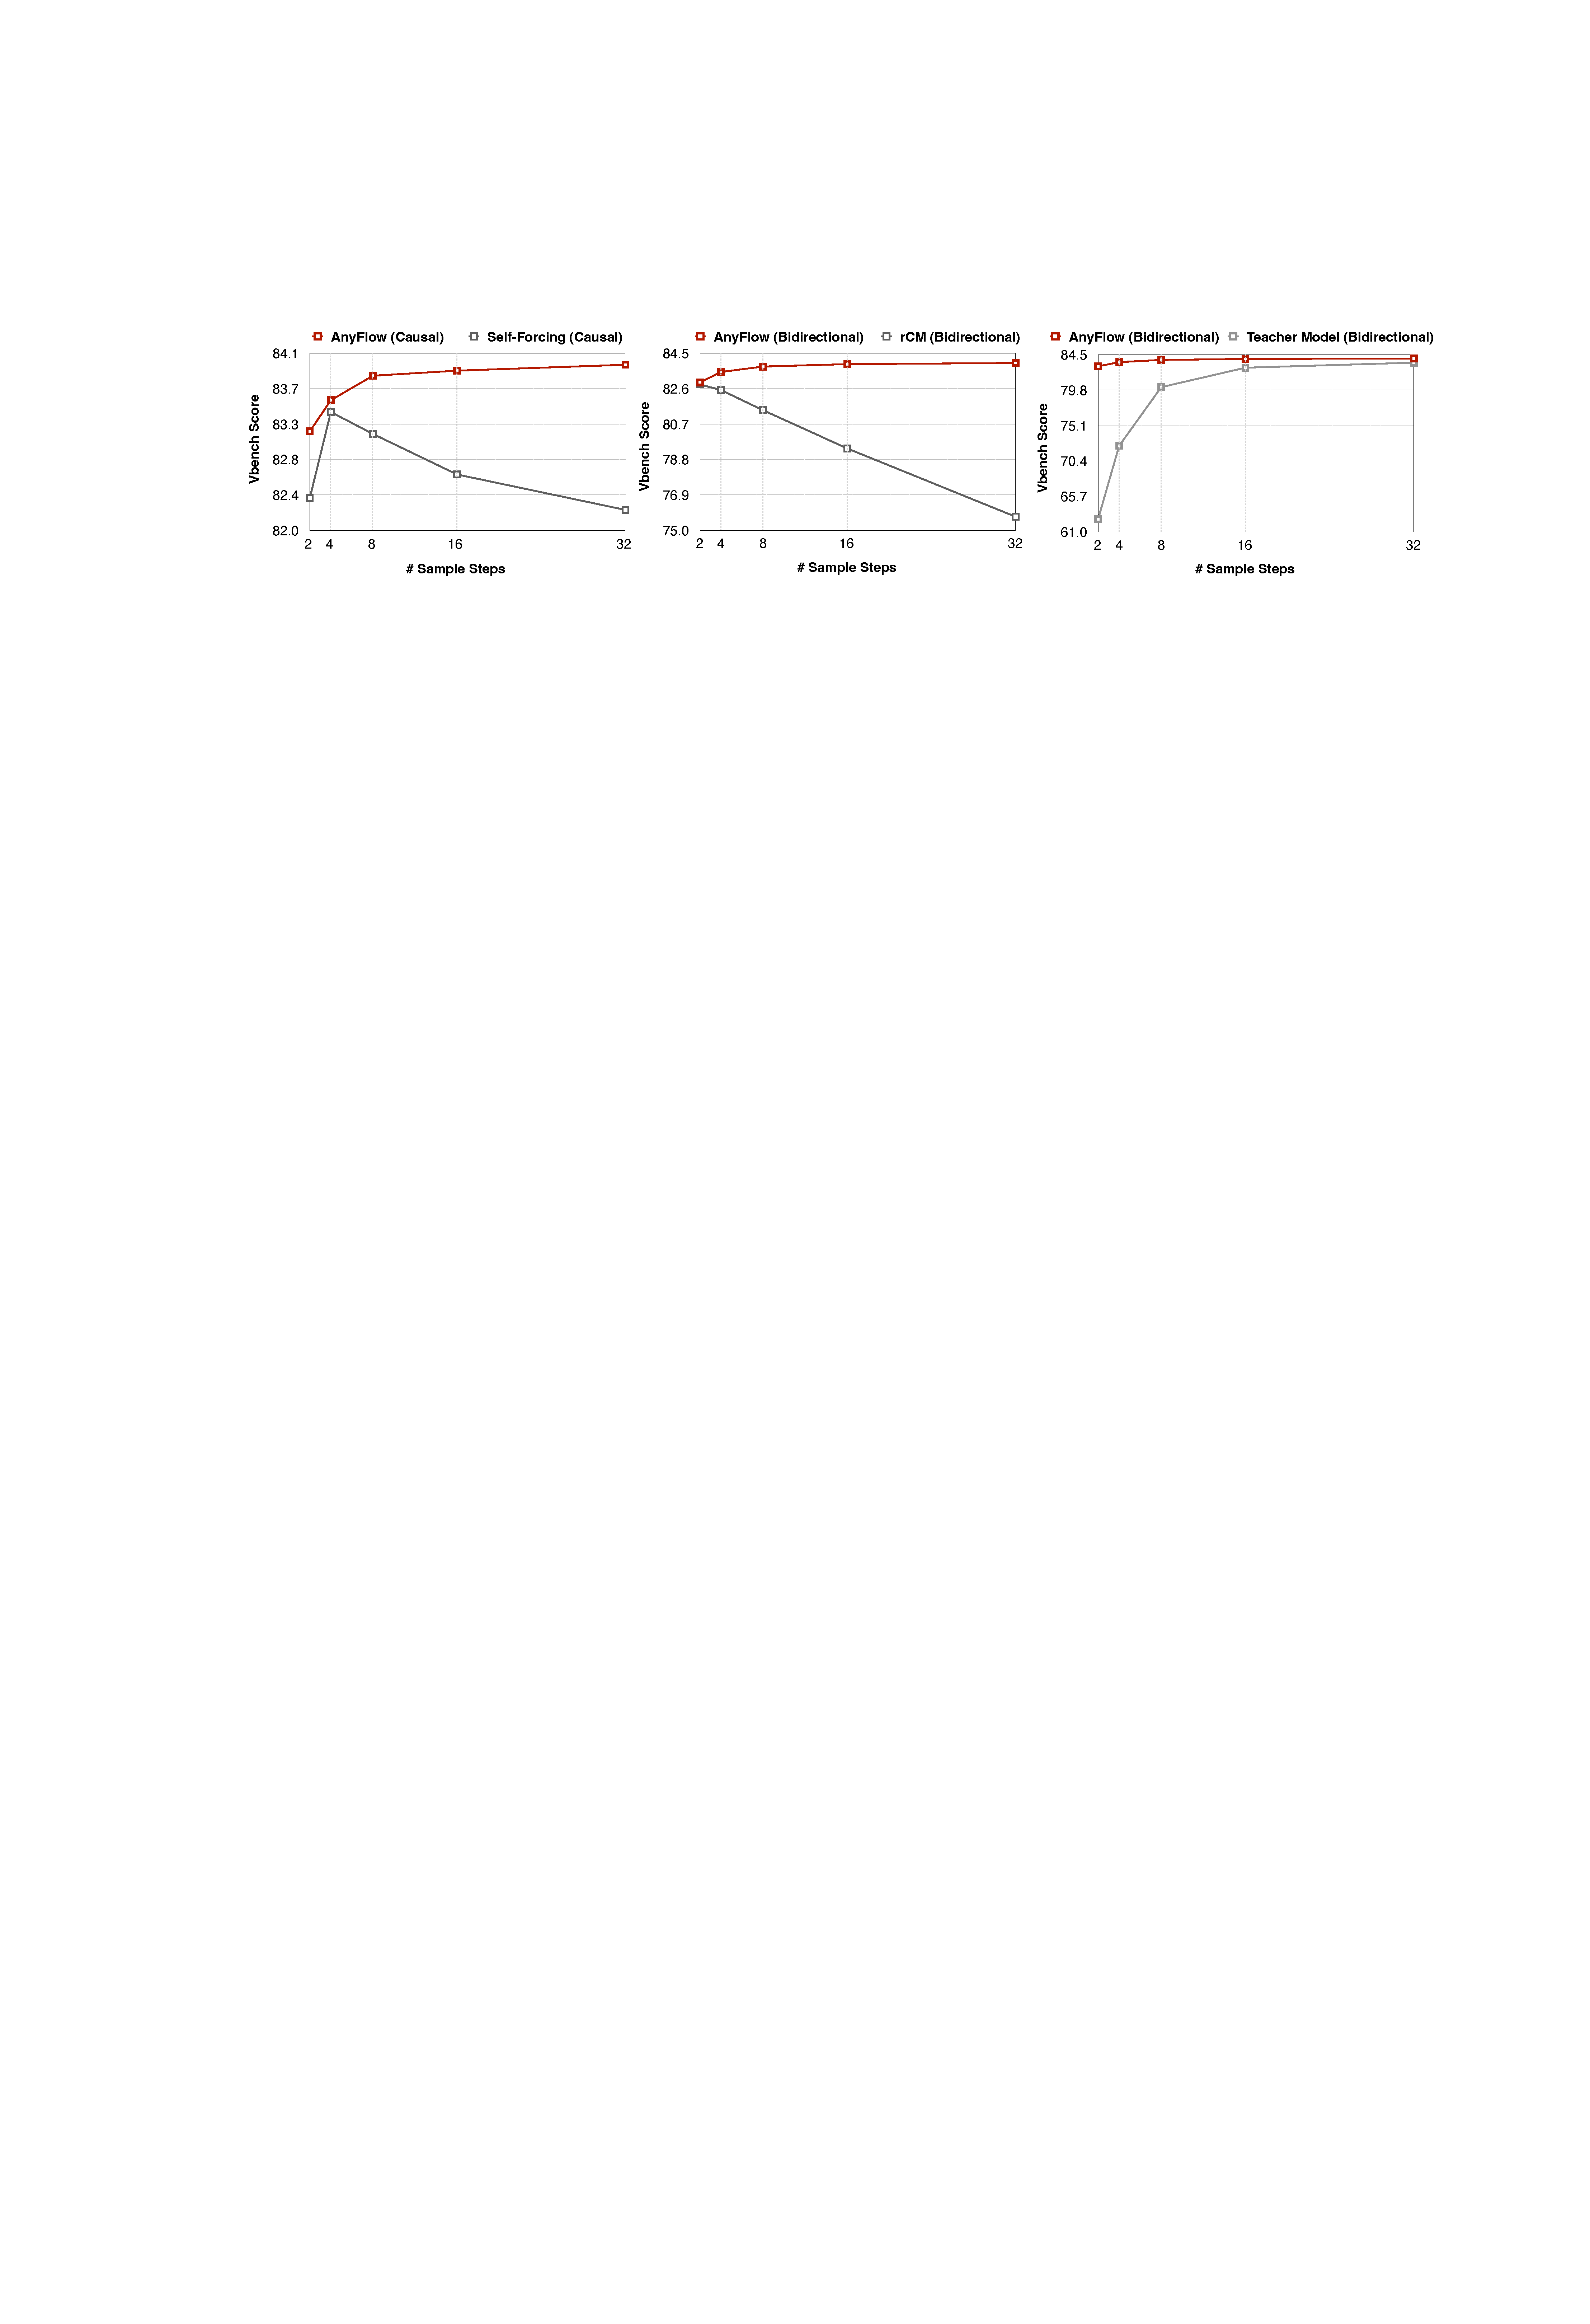
\includegraphics[width=\linewidth]{figures/src/teaser_test_scale.pdf}
    \caption{Quantitative comparison of AnyFlow test-time scaling against consistency-based methods and the teacher model.}
  \end{subfigure}
  \hfill
  \begin{subfigure}[b]{\linewidth}
    \centering
    \animategraphics[width=\linewidth]{8}{figures/videosrc/teaser/}{00000}{00020}
    \caption{Qualitative comparison of AnyFlow test-time scaling against consistency-based methods and the teacher model.}
  \end{subfigure}
  \caption{\textbf{Test-Time Scaling of AnyFlow.} Compared to consistency-based methods (\eg rCM~\cite{zheng2025large} for bidirectional video diffusion and Self-Forcing~\cite{huang2025selfforcing} for causal video diffusion), AnyFlow achieves strong performance in the few-step regime and scales effectively with increased sample steps. Compared to the teacher model, AnyFlow preserves test-time scaling ability while significantly improving the full trajectory. Readers can \textcolor{magenta}{click and play} the video clips in this figure using Adobe Acrobat.}
  \label{fig:teaser}
\end{figure*}


Specifically, AnyFlow contains two complementary stages. In the first stage, we develop an improved forward flow map training recipe to convert pretrained video diffusion models into flow map models, providing a strong initialization for any-step generation. However, forward flow map training alone cannot fully remove test-time errors: discretization error remains pronounced under low-NFE sampling, and exposure bias is still severe in causal generation. In the second stage, we introduce on-policy flow map distillation to optimize reverse divergence on model rollouts to mitigate test-time errors. The core design is flow map backward simulation, which replaces expensive full-trajectory simulation with shortcut decomposition, enabling efficient training of intermediate transitions over different time ranges. By combining forward flow map training with reverse-divergence supervision during on-policy distillation, AnyFlow achieves strong few-step quality while continuing to improve with more sampling steps. Moreover, because AnyFlow preserves the fine-grained flow field, the distilled model can be further adapted to downstream datasets through continued fine-tuning.

\begin{figure}[!tb]
  \centering
  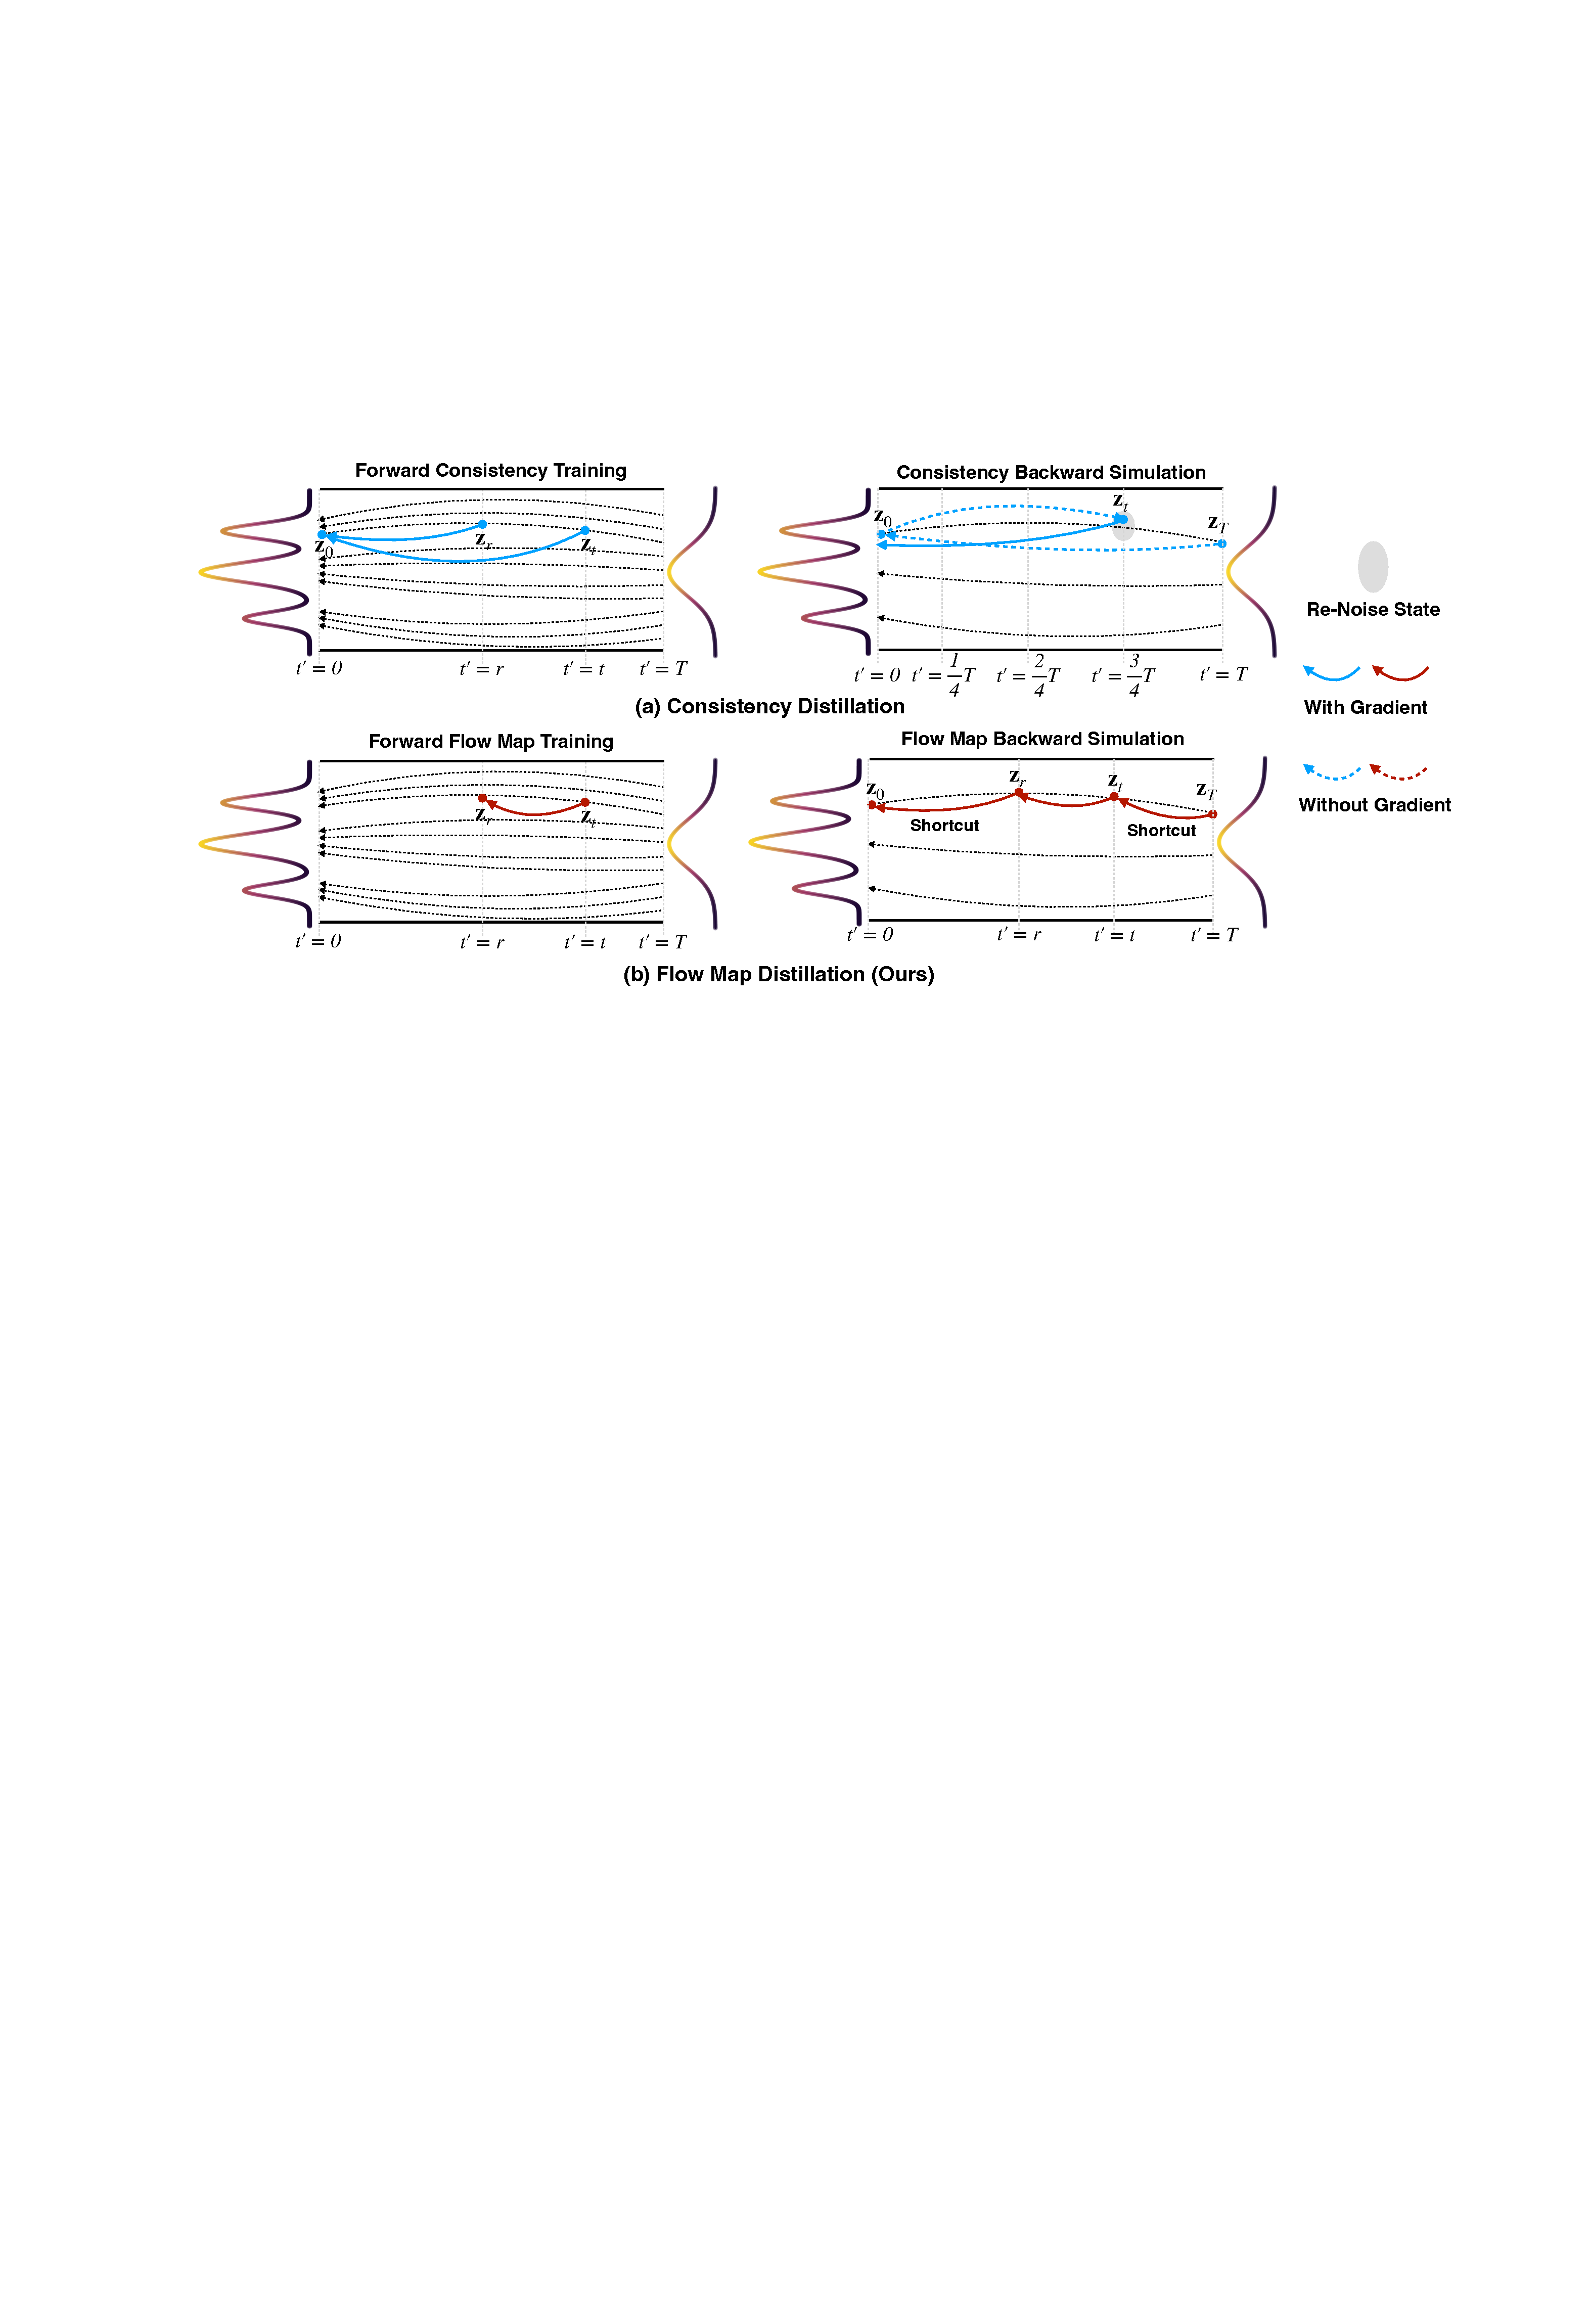
\includegraphics[width=\linewidth]{figures/src/paradigm_comparison.pdf}
  \caption{\textbf{Comparison of Distillation Paradigms.} (a) Consistency distillation learns a fixed-point mapping from $\mathbf{z}_t$ to $\mathbf{z}_0$. Its backward simulation requires re-noising intermediate states, which causes trajectory drift under multi-step sampling. (b) Flow map distillation learns transitions from $\mathbf{z}_t$ to $\mathbf{z}_r$. Its backward simulation decomposes Euler sampling trajectories into shortcut segments and enables efficient simulation of transitions across different step sizes.
  }
  \label{fig:paradigm_comp}
\end{figure}


We validate AnyFlow on both bidirectional and causal video diffusion models, ranging from 1.3B to 14B parameters. Across these settings, \textbf{AnyFlow matches or surpasses consistency-based counterparts even with few steps and continues to improve as the number of sampling steps increases}. In the causal setting, a single AnyFlow model jointly supports text-to-video, image-to-video, and video-to-video generation. For text-to-video, AnyFlow-FAR reaches 84.05 at 4 NFEs and further improves to 84.41 at 32 NFEs on the 14B model, surpassing Krea-Realtime-14B (83.25 at 4 NFEs). For image-to-video, AnyFlow-FAR achieves an 87.87 VBench-I2V score at 4 NFEs, comparable to Wan2.1-I2V-14B using 50$\times$2 NFEs (87.71). In the 14B bidirectional text-to-video setting, AnyFlow reaches 84.04 at 4 NFEs, outperforming rCM-14B (83.73 at 4 NFEs). Our contributions are summarized as follows:
\begin{itemize}
    \item We introduce AnyFlow, the first any-step video diffusion distillation framework built on flow maps, enabling a single model to support arbitrary inference budgets.
    \item We propose flow map backward simulation for on-policy flow map distillation to mitigate test-time errors (\ie discretization error and exposure bias) through efficient trajectory decomposition.
    \item We validate AnyFlow across architectures and model scales, establishing it as a scalable solution for high-quality, any-step video generation.
\end{itemize}
